\documentclass{article}
\usepackage{work}\usepackage{xcolor}
\usepackage{listings}
\usepackage{graphicx}
\usepackage{tikz}
\usetikzlibrary{automata, positioning}  
\usepackage{amsmath}
\def\title{Midterm 1 Review}
\lstset{ 
numbers = left,
  stepnumber=1,
  firstnumber = 1,
  numberfirstline = true,
  showstringspaces=false,
  language = Python 
  }
\begin{document}
\maketitle
\section{Introduction}
This worksheet will serve as a brief review of everything that has occurred in CS61A over the last few weeks. It is not comprehensive, but it should provide the high level overview that is required to gain intuition for most problems.
\section{Functions}
\textbf{Functions}, in the most basic sense, are a block of code, that can be used to perform some type of action. Functions have multiple uses, and can be used as return values, nested definitions, and arguments. 

\subsection{Structure}
\begin{lstlisting}[language = Python]
def hello(hi):
     ...
     return bye
\end{lstlisting}
In the above function, "hello" is the function name, hi is the argument and bye is the return value. 
Now that we've gone over the basics of functions, let's describe all of their use cases. \\*
\subsection{Functions as arguments}
Functions can be used as arguments. Let's take the following example: \\*
\bigskip
\begin{lstlisting}[language = Python]
def eatFood(makeFood):
     makeFood()
     print("I have eaten!")
\end{lstlisting}
Here we have a function \emph{eatFood}. In this, we have an argument, \emph{makeFood}. We call the function \emph{makeFood} and then say that "I have eaten!". Depending on the food that we want to eat, we will have a different method to make it. However, regardless of how we make the food, we will eat it the same way- with our mouths! Instead of making a new function for eating every type of food, we have a function for eating. This function takes in a function that makes our food, which makes a more universal function. 
\subsection{Returning Functions}
Say we wanted to make a function that allows us to eat cook some food given 1 ingredient and a set amount of time. At runtime, our function would take in a "mystery ingredient" and we would compare all the foods 
\begin{lstlisting}[language = Python]
func1 = makeFood(ravioli, x, 2)
func2 = makeFood(ice cream, x, 2)
func3 = makeFood(ravioli, x, 2211)
\end{lstlisting}
You can see why this can get a bit tiring, so instead of doing this, we can return a function. For the above example, we can make a function that takes in 3 arguments, the 2 food items, and the amount of time you want to cook them for. This looks as follows: 
\begin{lstlisting}[language = Python]
def checkFood(food1, time):
     return makeFood(food1, mystery, time)
\end{lstlisting}
Now our functions can be rewritten as 
\begin{lstlisting}[language = Python]
func1 = checkFood(ravioli, 2)
func2 = checkFood(ice cream, 2)
func3 = checkFood(ravioli, 2211)
\end{lstlisting}
The change isn't too obvious in this scenario; however, in times when you want some similar construction with different inputs (the x value), this process can save a lot of time. An example will come up when we deal with Nested Functions.
\subsection{Nested Functions}
Now that we have dealt with functions as return values and arguments, we will now deal with functions within functions. This concept can seem a bit overwhelming, but I promise, it will get a bit easier. Nested functions allow us to not have all the methods public to the global frame and it allows us to use the output of a specific function as the only possible input for a function. 
\begin{lstlisting}[language = Python]
def makeRavioli(time):
     def putSauce(flavor):
           print("put sauce")
     print("boiled it")
     return putSauce
\end{lstlisting}
Here we have a nested definition of \emph{putSauce}. We would not want people to put sauce on brownies, so it makes sense that this function would be within the \emph{makeRavioli} function. Additionally, if someone had some other pasta, they may want to have a \emph{putSauce} method that acts differently. Having nested definitions allows us to have methods with the same name and purpose that have different functionality.
\section{Recursion}
You are in a theater and want to know how many rows are in front of you but you can only see 1 row in front of you. To solve this problem, you ask the person in front of you “how many people are in front of you?”. They ask the person in front of them and this continues until reaching the person in the first row, they respond “0” to the person in the 2nd row. The person in the 2nd row knows there are 0 rows in the row in front of him, so he adds 1 to 0, 1, and tells guy behind him. That guy adds 1 to 1, 2, and tells guy behind him. This process repeats until you get back a number. This process is a real life application of the concept of \emph{recursion}. \\*
\bigskip
Recursion, in the most basic sense, is a function that calls itself, or other functions, and each time it does this, it simplifies the input problem until, it it simple enough to be solve trivially. Recursive algorithms consist of 2 main parts, the base case(s) and the the recursive call. A \emph{base case} is a conditional statement that that terminates the algorithm when invoked. The \emph{recursive step} is the call to the function that has a reduced input in order to solve the problem.
\begin{lstlisting}[language = Python]
def countdown(num):
     if(num ==1):
         return("bye")
     return countdown(num-1)
\end{lstlisting}
In the above function, line 2 contains the base case, where, if the num variable equals 1, then the algorithm terminates. Otherwise, we call the the function again on a smaller input. 

\subsection{Recursion between 2 functions}
We have dealt with functions that call themselves; however, in recursion, sometimes we call other functions, and use them to make our input smaller.
\begin{lstlisting}[language = Python]
def countdown(num):
     if(num ==1):
         return("bye")
     return countdown(num-1)
def divide(num):
     if(num == 1):
          return("hi")
     return countdown(num/2)
\end{lstlisting}
In the above example, the recursive step of \emph{countdown} returns the output of the function \emph{divide} with an input of num - 1. The recursive step of \emph{divide} returns the output of the function \emph{countdown} with an input of num/2. These functions can be particularly useful when we want to alternate between 2 steps. 

\subsection{Recursion going up}
Recursion is not always as simple as just going down, sometimes, once your algorithm terminates, we need to "go up" as well. This can occur when there are steps after or including the recursive call. 
\begin{lstlisting}[language = Python]
def sumSquares(n):
     if(n == 1):
         return 1
     return pow(n,2) + sumSquares(n-1)
\end{lstlisting}
In the above function, we are attempting to find the sum of the squares of the first n natural numbers. At each step on the way down, we add n square to the return value of the sumSquares(n-1). For example, for take sumSquares(3). The return value of this function is 9 + sumSquares(2), for sumSquares(2) the return value would be 4 + sumSquares(1), and for 1, the base case holds so the return value is 1. \\*
\bigskip
From here, we essentially perform a series of substitutions. We substitute 1 for sumSquares(1) which gets up 4+ 1 = 5 for sumSquares 2. We then substitute this value into sumSquares(2) and get 9 + 5 =14 for sumSquares(3) return value. At this point, we have exhausted all the steps that we must perform and we return 14. \\*
\bigskip
This process is equivalent to the following environment diagrams  \\*
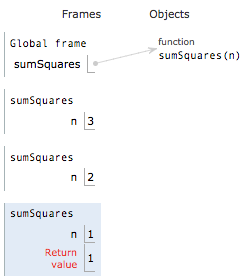
\includegraphics[scale=.6]{../images/frame1.png}{\Huge $\rightarrow$}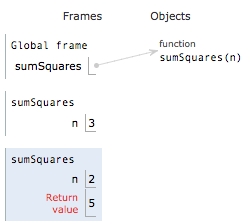
\includegraphics[scale=.6]{../images/frame2.png} {\Huge $\rightarrow$} 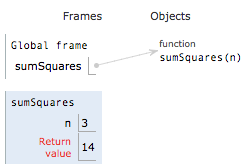
\includegraphics[scale=.6]{../images/frame3.png} \\*
Note that the first frame is for the return value of \emph{sumSquares(1)}, the 2nd for \emph{sumSquares(2)}, and the 3rd for \emph{sumSquares(3)}.
\subsection{Tree Recursion}
Tree Recursion is the process when a function that calls itself more than once during one step. For example: 
\begin{lstlisting}[language = Python]
def walkSteps(n):
     if(n <= 2):
         return n
     return walkSteps(n-1) + walkSteps(n-2)
\end{lstlisting}
In this function, we are counting the amount of ways that we can walk on a certain path of distance n steps, where you can walk either 1 step or 2 steps at a time. We will walk through the example of n =3. We return walkSteps(2) + walkSteps(1). We then return n for each one of these case, since from 2 there are 2 ways to reach the end by walking 2 steps once or 1 step twice, and from 1 there is 1 way to reach the end. We add these 2 cases and get a total of 3 ways to walk the path. \\*
\bigskip
At each step, you see the paths that will occur if you take 1 step or 2 steps. Once you reach a distance of 2 or less steps from the end, you simply return n. 
\section{Environments}
In CS61A we deal with \emph{environment diagrams} which help us visualize how we can walk through a program, we will discuss how to think about each step in an environment diagram.
\subsection{Basics of Environments}
\emph{Variables} in Python can be thought of as a storage location for anything, from a function to a number to a string. Variables take the following form \\*
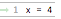
\includegraphics[scale=.7]{../images/var1.png}{\Huge $\rightarrow$}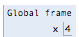
\includegraphics[scale=.7]{../images/var2.png} \\*
The item on the left side of the equals is the variable and the item on the right side is the value that it is taking on. \\*
\bigskip
There are 2 types of major types functions in Python, \emph{user defined functions} and \emph{Non-user defined functions}. A user defined function is a function that the user builds that takes in some set variables. \\* 
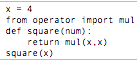
\includegraphics[scale=.7]{../images/user1.png}{\Huge $\rightarrow$}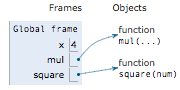
\includegraphics[scale=.7]{../images/user2.png} \\* \bigskip

In the above set of calls, \emph{mul} is something defined from operator and \emph{square} is a user defined function. Note how in the frames, mul takes in an arbitrary amount of arguments labeled as "..." whereas \emph{square} takes in only 1 argument.
\subsection{Frames}
\emph{Frames} can be thought of as a way to keep track of a function call in progress. We will examine a function and pick apart frames and their attributes.
\\* 
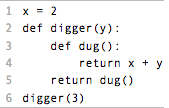
\includegraphics[scale=.7]{../images/dug1.png}{\Huge $\rightarrow$}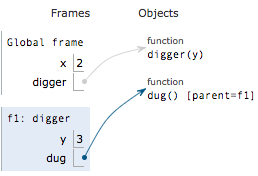
\includegraphics[scale=.7]{../images/dug2.png} \\* \bigskip
 The \emph{Global Frame} is a frame that has no parent, and every variable or function is either in the global frame or some sub frame. A \emph{Parent Frame} is the frame which a function is defined in. In the above function, x and \emph{digger} are defined in the Global Frame. The function \emph{dug} has a parent in frame 1, or our call to \emph{digger} with the argument 3. 
 
 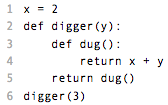
\includegraphics[scale=.7]{../images/dug3.png}{\Huge $\rightarrow$}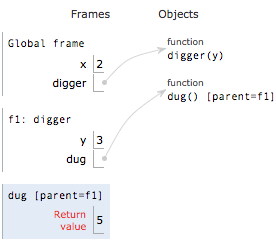
\includegraphics[scale=.7]{../images/dug4.png} \\* \bigskip
 When we completed our call in \emph{dug}, we see that even though we did not define x and y in the frame, it still managed to complete without error! We will discuss why this is in the next lesson. 
 \subsection{Scope}
 In the earlier section, confusion may have arisen when somehow our variables gained access to other ones? How do we know which variables we can use? Well there are a fixed set of rules about variables and their accessibility.
\begin{itemize}
\item You can only access variables in scopes that are above the current frame. 
\item You cannot modify the variable in a lower scope. You can only get its value
\item A variable can only be defined once in a scope (no variables with 2 names defined in the same scope).
\item If 2 variables have the same name and are defined in different scopes, the one that is closer will be used as the value
\item A function's variables have the value of the scope that it was defined in.
\end{itemize}
That was a lot of rules, so lets go over some examples when the rules would hold. 
\begin{lstlisting}[language = Python]
def eat():
     hunger = false
eat()
appetite = hunger
\end{lstlisting}
This block of code would error out because appetite is in the frame above the frame that hunger would be defined in. As a result, we cannot set appetite equal to it. Mainly because there is the parent frame has no clue about what is below it. A way to get around this is as follows. 
\begin{lstlisting}[language = Python]
def eat():
     hunger = false
     return hunger
appetite  = eat()
\end{lstlisting}
We modified our code so that appetite would be equal to the return value of \emph{eat}. Since eat returns false, appetite would be false. 
\begin{lstlisting}[language = Python]
energy = 10
def work():
     energy--
work()
\end{lstlisting}
This above code would error out because we cannot directly modify the energy variable in a frame below it. What you can do is make a variable, set it equal to energy and then modify that. That is done as follows. 
\begin{lstlisting}[language = Python]
energy = 10
def work():
     lifeforce = energy
     lifeforce--
work()
\end{lstlisting}
This would run properly; however, if you wanted to change the value of energy, you would need to do something similar to out fix in the prior problem. 
\begin{lstlisting}[language = Python]
energy = 10
def work(x):
     x--
     return x
energy = work(energy)
\end{lstlisting}
Here we can modify the energy variable by setting it equal to the result of the work method. 
\begin{lstlisting}[language = Python]
x = 2
x = 3
\end{lstlisting}
In this case, no real error occurs. Basically all that is happening is that the variable x is associated with 3 and not x once the program is completed.  \\*
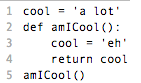
\includegraphics[scale=.7]{../images/cool1.png}{\Huge $\rightarrow$}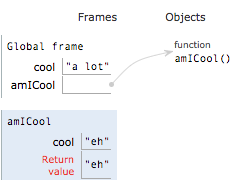
\includegraphics[scale=.7]{../images/cool2.png} \\* \bigskip
In this example, we have the variable \emph{cool} defined in the global frame. Then when we call \emph{amICool} it returns "eh. That is because we defined a second cool in that frame that is closer to our call of cool. \\* \bigskip
The last rule is the one that most people consider a bit more confusing. \\* \bigskip

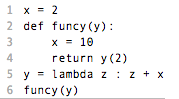
\includegraphics[scale=.7]{../images/funcy1.png}{\Huge $\rightarrow$}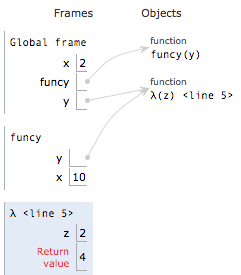
\includegraphics[scale=.7]{../images/funcy2.png} \\* \bigskip
In the above function, we have a lambda function that is defined in the global frame. We then pass it into out function \emph{funcy} and attempt to evaluate it. We pass in the value 2 as the argument for z; however, when it comes to choosing the value for x, \textbf{we do not go to the frame that the function was evaluated in, instead we pick the value of x based off where the function was defined}. If x was not defined in the global frame, there would be an error. 
\section{Misc.}
Here I will discuss miscellaneous categories that are in the first unit of CS61A that tend to be a bit tricky
\subsection{Lambda Functions}
Lambda function are a concise way to write definition statements.
\begin{lstlisting}[language = Python]
def func1(x):
     return 10
\end{lstlisting}
The above example is equivalent to 
\begin{lstlisting}[language = Python]
lambda x : 10
\end{lstlisting}
Realize that there is a 1 to 1 correspondence between lambda function and def statements. Rewriting lambda's in a much more well known form can really aid in the understanding of these types of problems.

\subsection{The Print Function}
The print function is one that is really unique. It displays something to the user output; however, the value of a print is always None. For example: 
\begin{lstlisting}[language = Python]
def print10():
     x = print(10)
     return x
\end{lstlisting}
This function would first print 10 then bound x to the return value of the print statement. This is always None, regardless of the input to the print function.
\\* 
\bigskip
Additionally, returning and printing a string would yield different outputs. Printing a string would always result in the said string having no quotes around it; however, if you returned a string, there would be quotes around it. For example: 
\begin{lstlisting}[language = Python]
def returnStr():
     return "hello"
returnStr()
\end{lstlisting}
returns 'hello'. While 
\begin{lstlisting}[language = Python]
def printStr():
     print "hello"
printStr()
\end{lstlisting}
prints hello. You do not really need to know why this occurs, but it is an interesting fact to keep in mind. \\*

\newpage
\Question{Butter Nutter}
\begin{subq}
 \subqs Label the parts of the following function: 
 \lstinputlisting[language=Python, firstline=1, lastline=11]{../code/environments.py}
  \bigskip
 
\begin{solution}

\lstinputlisting[language=Python, firstline=15, lastline=23]{../code/environments.py}
 \end{solution}
 \subqs What does the above code snippit return? 
 \begin{solution}
 strawberrycrunchy
 \end{solution}
\end{subq}
\Question{Goats and Lambs}
\begin{subq}
\subqs Lambdas are very niche functions. They are used to write short, one line def statements.  Write the following lambda statement as a normal def statement function. lambda x:  lambda y : lambda z: x + y + 1
\begin{solution}
\begin{lstlisting}[language = Python]
def func1(x):
     def func2(y):
          def func3(z):
                return x + y + 1
          return func3
     return func(2)
\end{lstlisting}\end{solution}

\subqs Write the following function as a lambda: 
\begin{lstlisting}[language = Python]
def fib(n):
     if(n < =1):
          return n
     else:
          return fib(n-1)+ fib(n-2)
\end{lstlisting}
\begin{solution}
fib = lambda n: n if n $<=$1 else fib(n-1)+fib(n-2)

\end{solution}
\subqs Within 4 lines create a function or set of functions that do the following: 
You are given an integer input. If n, the number of digits, in the integer is odd find n factorial. Otherwise, find the nth fibonacci number
\begin{solution}
\begin{lstlisting}[language = Python]
dig = lambda x: 1 if x < 10 else 1 + dig(x//10)
fib = lambda x: x if x <=2 else fib(x-1) + fib(x-2)
fact = lambda x : 1 if x<=1 else x*factorial(x-1)
func1 = lambda x: fib(dig(x)) if dig(x)%2 == 0 else fact(dig(x))
\end{lstlisting}
\end{solution}
\end{subq}
\newpage



\end{document}